\og \textit{la Croix, signe d’espérance} \fg

Bien conscient du drame qui se trame contre lui et le bouleverse au plus profond de son être à l’approche de son ‘‘heure’’, Jésus décide pourtant d’aller jusqu’au bout du don de soi. Si au plan des relations humaines, en ce qui fait la valeur de l’homme c’est sa réussite sociale, aux yeux de Dieu l’homme ne vaut que par sa capacité de don. 

C’est bien ce qu’a été toute la vie de Jésus. Dans le don de sa vie, il a obéi à son Père jusqu’à la croix. C’est en cela que la croix reste pour nous les chrétiens un mystère. La victoire de la croix, la victoire de l'amour sur la haine et la violence, de la vérité sur le mensonge, de la vie sur la mort, demeure encore pour le mystère de notre rédemption. 

Dans le monde règnent encore aujourd'hui la haine, le mensonge et la violence. La vie nouvelle ne nous est donnée que sous la forme de la croix. "L'histoire de l'espérance, dans laquelle Jésus se manifeste comme le Fils de Dieu vivant pour toujours, n'est pas une série continue de succès, ni un récit de victoires à l'échelle humaine". C'est au bout du chemin de la croix que nous est promise la victoire de la croix. Car c'est précisément la kénose, c’est-à-dire l'abaissement de Dieu, jusque dans l'abîme de la souffrance et de la mort où nous sommes plongés, qui nous a de nouveau unis à Dieu dans cette situation concrète qui est la nôtre. Ainsi la croix est-elle signe de l'espérance que nous serons un jour totalement libérés et que Dieu définitivement règnera sur le mal.

Dès lors,
prendre notre croix quotidienne signifie nous engager dans la logique paradoxale du renoncement à soi pour le règne grandisse en nous.
\begin{wrapfigure}{l}{1.5cm}
\vspace{-0.5cm}
	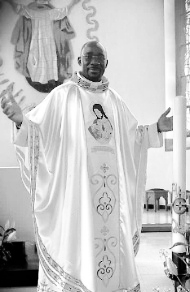
\includegraphics[scale=1.2]{standing_daniel.png}
\end{wrapfigure}
Si nos sociétés sont si facilement prisonnières de la violence et des hostilités fratricides c’est parce qu’elles sont régies par la mentalité de l’égoïsme absolutisé : tout ce qui n’est pas fait pour soi semble être une perte, un échec. Seul l’intérêt, avoué ou caché, semble faire mouvoir le monde. Et pourtant c’est le don de 
soi qui libère, c’est l’amour qui sauve le monde, c’est de la Croix que jaillit la vie nouvelle.                                                                                                                                                                

\begin{flushright}
Bonne montée vers Pâques !\\
\textit{Père  Daniel  ETTÉ}
\end{flushright}
